\documentclass[xelatex,ja=standard,jafont=noto]{bxjsarticle}
\usepackage{kyremath}

\title{calculus-semi}

\author{Kyure\_A}

\date{\today}

%--------------------------------------------------------------------------------------------------------

\begin{document}
 
 \maketitle

 \section*{諸注意}
 言い訳がましいが,俺は論理記号がエアプなのでイキって間違った記述をしている場合がある.説明と異なるような記述があれば,適宜指摘をお願いしたい.また,書けるところは論理記号で書いていたり,書けないところは普通に日本語を用いて書いていたりするので表記の不統一が散見されると思う.
 あと普通に書いてから 1 ヶ月経過した結果かなり内容を忘れている (6/25)

 \tableofcontents
 \clearpage

 \section{実数と数列}

  \subsection{実数の連続性}

  \begin{tcb}{上界と下界}{}
   \begin{itemize}
    \item 上界 

	  $\forall x \in S, x \leq a$ ならば, $a$ を $S$ の上界という.

    \item 下界 

	  $\forall x \in S, a \leq x$ ならば,$a$ を $S$ の下界という.

   \end{itemize}
  \end{tcb}
  
  また,$S \subset \mathbb{R}$ が上界をもつとき,S を上に有界であるといい,S が下界をもつときは下に有界であるという.また,これら両方をもつとき S は有界であるという.(上/下界を "持つ" だとだめっぽい?)

  ここで,$S \subset \mathbb{R}$ に対して,その上界全体の集合を U(S), 下界全体の集合を L(S) と表すこととする.
  このとき,U(S), L(S) を論理記号を用いて表すと
  \begin{tcb}{U(S), L(S) の定義}{}
   \centerline
   {$
   U(S) = \{a \mid \forall x \in S (x \leq a)\}
   $}
   \centerline
   {$
   L(S) = \{a \mid \forall x \in S (a \leq x)\}
   $}
  \end{tcb}
  となる.つまり,S が 上界を持つ $\Leftrightarrow U(S) \neq \emptyset$  であるし,S が下界を持つ $\Leftrightarrow L(S) \neq \emptyset$ である.
  
  \pagebreak

 \begin{tcb}{上限と下限}{}
  \begin{itemize}
   \item 上限 (supremum)

	 $S \subset \mathbb{R}$ が上に有界である,その上界の中で最小の $x \in \mathbb{R}$ が存在するならば, $x$ を $S$ の上限であるといい,記号 $\sup S$ で表す.つまり,$U(S)$ があって $\min U(S)$ が存在するならば,それを $\sup S$ と表す.

   \item 下限 (infimum)

	 $S \subset \mathbb{R}$ が下に有界である,その下界の中で最大の $x \in \mathbb{R}$ が存在するならば,$x$ を $S$ の下限であるといい,記号 $\inf S$ で表す.つまり $L(S)$ をもつとき,$\max L(S)$ が存在するならば,それを $\inf S$ と表す.

  \end{itemize}
 \end{tcb}

 閉区間の集合 $[a, b]$ と開区間の集合 $(a, b)$ を考える.両者ともに区間の左端が a で,右端が b である.前者には最小値 a, 最大値 b があるが,後者には最小値も最大値も存在しない.しかし,両者はともに有界であるため,上限と下限について考えることができる.実際,$\forall x \in [a, b]$ について $ a \leq x$ であるし,$\forall x \in [a, b]$ について $x \leq b$ である.(後者に関しては,$<$ と読み替えればよい) \\ したがって,上限と下限の概念は最小値と最大値の概念よりもより広範に適用できる概念であるっぽい.

 \begin{tcb}{上限と下限の性質}{}

  \begin{enumerate}
   \item 上に有界な集合 S について,$a = \sup S$ であることは次の条件がともに満たされることである.
	 \begin{itemize}
	  \item[(a) ] $\forall x \in S$ について $x \leq a$ である.
	  \item[(b) ] $a' < a$ ならば,$\exists x \in S, a' < x$ である.

		      つまり,$a$ より小さい上限 $a'$ を仮定しても,$a'$ より大きい $x \in S$ が存在しているよということである.
	 \end{itemize}
   \item 下に有界な集合 S について,$a = \inf S$ であることは次の条件がともに満たされることである.
	 \begin{itemize}
	  \item[(a) ] $\forall x \in S$ について $a \leq x$ である.
	  \item[(b) ] $a' > a$ ならば,$\exists x \in S, a' > x$ である.

		      つまり $a$ より大きい下限 $a'$ を仮定しても,$a'$ より小さい $x \in S$ が存在しているよということである.
	 \end{itemize}
  \end{enumerate}

 \end{tcb}

 次に,$S, T \subset \mathbb{R}, S \subseteq T$ である状況を考える.このときの $\sup S$ と $\sup T$ について,$a $ が $S$ の上界ならば,$\forall x \in S$ について $x \leq a$ だし,$\forall x \in T$ について $x \leq a$ である.よって $S$ の上界はすべて $T$ の上界でもあることがわかるから,$U(S) \subseteq U(T)$が成り立つ.同様に $\inf S$ と $\inf T$ についても考えられる.\\ \\
 よって
 
 \begin{tcb}{$S \subseteq T$ であるときの $\sup$ と $\inf$}{}
  \centerline{$S \subseteq T$ ならば,$\sup T \geq \sup S$}
  \centerline{$S \subseteq T$ ならば,$\inf S \leq \inf T$}
 \end{tcb}
これらの関係は以下のように数直線上に表すとわかりやすい.

\centerline{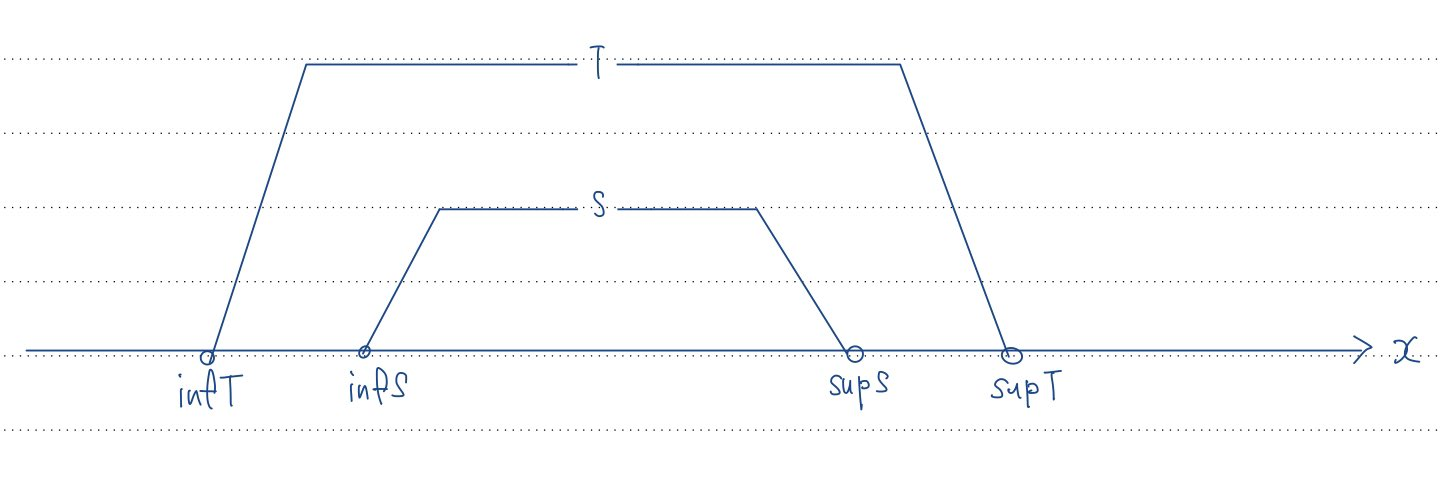
\includegraphics[width= 10cm]{./GYPtkDEb.jpg}}
   
   \subsubsection{実数の連続性}
   稠密性と連続性についてあやふやな理解をしていた.直感的に考えて $\mathbb{Q}$ にも $\mathbb{R} \setminus \mathbb{Q}$ にも数直線上で表すと隙間がある,つまり連続ではないことはわかっていたが,連続 $=$ 稠密だと思っていたのでこれらは稠密ではないと思っていた.しかし,連続性と稠密性は全く違った概念である.これらの数直線は稠密であるが,連続ではないらしい.一方,$\mathbb{R}$ は連続であり稠密である.\\
   参考にした「大学教養 微分積分」ではデデキント切断とかいう名前だけはよく聞く概念による実数の連続性の定義は書かれておらず,以下の公理を認めて議論を展開するとしている.

   \begin{axiom}{実数の連続性公理(Weierstrass の公理)}{}
    \begin{itemize}
     \item $S \subset \mathbb{R}$が上に有界であるとき,$\sup S$ が存在する.
     \item $S \subset \mathbb{R}$ が下に有界であるとき,$\inf S$ が存在する.
    \end{itemize}

   \end{axiom}

実数の連続性公理から以下が得られる.
  \begin{corollary}{アルキメデスの原理}{}
   \begin{itemize}
   \item $ \forall a \in \mathbb{R} _ {++}$ (正の実数) と $\forall b \in \mathbb{R}$ に対して,$an > b$ となるような $n \in \mathbb{N}$ が存在する.

   \end{itemize}
  \end{corollary}
「アルキメデスの原理」という語は物理で一般に使われているが,「大学教養 微分積分」によるとこれも「アルキメデスの原理」らしい.

  \begin{proof}{アルキメデスの原理の証明(写経)}{}

   背理法で証明する.アルキメデスの原理の原理が成り立たないと仮定すると,$\forall n \in \mathbb{N}$ について $an \leq b$ すなわち $n \leq \frac{b}{a}$ を満たす $a \in \mathbb{R}_{++}$ と $b \in \mathbb{R}$ が存在する.よって実数の連続性公理から $\mathbb{N}$ は上に有界であり,$\sup \mathbb{N}$ が存在する.また,$\sup \mathbb{N} - 1$ は $\mathbb{N}$ の上界ではないので,$\sup \mathbb{N} - 1 < m$ となる自然数 $m$ が存在する.このとき,$\sup \mathbb{N} < m + 1$ であるから,$\sup \mathbb{N}$ より大きい自然数 $m + 1$ が存在する.このことは,$\forall n \in \mathbb{N}$ について $n \leq \sup \mathbb{N}$ であることに矛盾する.

  \end{proof}


 公理1.2 の不等式の両辺を n で割ると以下の系が得られる.

  \begin{corollary}{}{}
   任意の正の実数 a と 実数 b に対して,$a > \frac{b}{n}$ となる自然数 n が存在する.
  \end{corollary}

  \begin{theorem}{有理数の稠密性}{}
   空集合でない開区間の中には,少なくとも一つの有理数が存在する.
  \end{theorem}

  \begin{proof}{有理数の稠密性の証明(写経)}{}
   開区間 $(a, b) (a < b)$ を考える.$a < 0 < b$ ならば,開区間$(a, b)$ は有理数 $0$ を含む.$a < b < 0$ のとき,開区間 $(-b, -a)$ が有理数 $r$ を含む,つまり $-b < r < -a$ ならば,開区間$(a, b)$ は有理数 $-r$ を含む.よって $0 < a < b$ のときを証明すればよい.$b - a \in \mathbb{R}$ と自然数 $1$ に対して,アルキメデスの原理より,$(b - a)n > 1$ となる $n \in \mathbb{N}$ がとれる.これを変形すると $a + \frac{1}{n} < b$ であることがわかる.次に,$\frac{1}{n}, a \in \mathbb{R}$ に対して,アルキメデスの原理より $\frac{1}{n}m > a$ となる自然数 $m$ がとれる.これが成り立つような最小の$m$をとれば,$\frac{m - 1}{n} \leq a < \frac{m}{n}$ となる.このとき,$a < \frac{m}{n} = \frac{m - 1}{n} + \frac{1}{n} \leq a + \frac{1}{n} < b$ である.よって,$a < \frac{m}{n} < b$ であるから,$\frac{m}{n}$ が開区間 $(a, b)$ に属していることがわかる.(このとき,$(b-a)n > 1$ を満たす $n $を無数に取ることができる.)

  \end{proof}
   \begin{corollary}{}{}
    $\forall \alpha \in \mathbb{R}$ と $\varepsilon \in \mathbb{R}_{++}$ に対して,$|\alpha - a| < \varepsilon$ を満たす $a \in \mathbb{Q}$ が少なくとも一つ存在する.

   \end{corollary}
 これは,$\alpha$ が無理数であるときに,$\alpha$ にいくらでも近い(ここガバ)有理数 a が取れることを示している.

  \subsection{数列の収束と発散}

  \begin{tcb}{極限}{}

   $\forall \varepsilon \in \mathbb{R}$ に対して,ある自然数 $N$ が存在して,$n \geq N$ であるすべての自然数 $n$ について,$|a_n - \alpha| < \varepsilon$ となるとき,数列 $\{a_n\}$ は $\alpha$ に収束するという.\\
   このとき,$\lim_{n \to \infty} a_n = \alpha$ または $n \to \infty$ のとき $a_n \to \alpha$ と表す.この値 $\alpha$ を数列 $\{a_n\}$ の極限値という.$\{a_n\}$ の極限は $\alpha$ であるともいう.\\
   \\
   また,数列 $\{a_n\}$ が収束しないとき,$\{a_n\}$ は発散するという.\\
   \\
   任意の実数 $M$ に対して,ある自然数 $N$ が存在して,$n \geq N$ となる任意の自然数 $n$ について $a_n > M$ なるとき,数列 $\{a_n\}$ は正の無限大に発散する,数列$\{a_n\}$の極限は正の無限大であるといい,$\lim_{n \to \infty} a_n = \infty$ または $n \to \infty$ のとき $a_n \to \infty$ と表す.\\
   \\
   任意の実数 $M$ に対して,ある自然数 $N$ が存在して,$n \geq N$ となる任意の自然数 $n$ について $a_n < M$ なるとき,数列 $\{a_n\}$ は負の無限大に発散する,数列$\{a_n\}$の極限は負の無限大であるといい,$\lim_{n \to \infty} a_n = -\infty$ または $n \to \infty$ のとき $a_n \to -\infty$ と表す.

  \end{tcb}

  \begin{tcb}{$\varepsilon - N$ 論法}{}
   「数列の収束について,正の実数 $\varepsilon$ が与えられたとき,$N \leq n$ となる任意の自然数 $n$ について $|a_n - \alpha| < \varepsilon$ が成り立つような $N$ を $\varepsilon$ を用いて作ることで議論する方法」を指す.このとき,$N$ は $\varepsilon$ に依存していると考えるとわかりやすい. 

  \end{tcb}
 手始めに,まずは $\lim_{n \to \infty} \frac{n}{n + 1} = 1$ となることを $\varepsilon - N $論法を用いて示す. 

  \begin{tcb}{$\varepsilon - N$ 論法の例 1: 収束を示す}{}
   取り敢えず,やりたいことは「$N < n$ である任意の自然数 $n$ について $|\frac{n}{n + 1} - 1| < \varepsilon$ が成り立つような $N$ が存在することを示す」ということだ.
   \\
   \\
   任意の正の実数 $\varepsilon$,自然数 $m$ に対して,$|\frac{m}{m + 1} - \frac{m + 1}{m + 1}| < \varepsilon \Leftrightarrow |\frac{-1}{m + 1}| < \varepsilon \Leftrightarrow  \varepsilon  > \frac{1}{m + 1}$ である.このとき,$m + 1 \stackrel{\mathrm{def}}{=} N$ とすると $N$ 以上のすべての自然数 $n$ について,$|\frac{n}{n + 1} - 1| = \frac{1}{n + 1} \leq \frac{1}{N} < \varepsilon$ である.以上より,任意の正の実数 $\varepsilon$ に応じて,$N$ 以上の任意の $n$ について $|\frac{n}{n + 1} - 1| < \varepsilon$ が成り立つような $N$ が取れることが示された.

  \end{tcb}

 また,$\varepsilon - N$ 論法は数列が収束しないことを証明すること,無限大に発散することを厳密に定義することにも使える.
  \begin{tcb}{$ \varepsilon - N$ 論法の例 2: 振動を示す}{}
   数列 $\frac{(-1)^n}{2} = \{a_n\}$ がある実数 $\alpha$ に収束するとして,
   数列 $\{a_n\}$ が $\alpha$ に収束する条件を,特に $\varepsilon = \frac{1}{2}$ のときに適用する.このとき,ある $N$ が存在して,$N \leq n$ である任意の自然数 $n$ に対して $|a_n - \alpha| < \frac{1}{2}$ となる.
   \\
   $n$ が奇数のときは,$a_n = \frac{-1}{2}$ であるから,$|\frac{-1}{2} - \alpha| = \frac{1}{2} + \alpha < \frac{1}{2}$ となる.このとき,$\alpha < 0$ である.
   \\
   $n$ が偶数のときは,$a_n = \frac{1}{2}$ であるから,$|\frac{1}{2} - \alpha| = \frac{1}{2} - \alpha < \frac{1}{2}$ となる.このとき,$\alpha > 0$ である.
   これは矛盾しているため,数列 $\{a_n\}$ がいかなる実数値 $\alpha$ にも収束しない.

  \end{tcb}

   \begin{tcb}{$ \varepsilon - N$ 論法の例 3: 正の無限大への発散を示す}{}
    数列 $\{a_n\} = 2n$ がある実数値$ \alpha$ に収束するとして,アルキメデスの原理より,$2n$ と任意の正の実数 $\varepsilon$ に対して,$\varepsilon m > 2n$ となるような自然数 $m$ が存在する. (途中)

   \end{tcb}

  \begin{theorem}{極限の一意性}{}
   数列 $\{a_n\}$ が収束するとき,その極限値は一意に定まる.
  \end{theorem}

「収束」という言葉の意味について考えると当たり前のことだが,これについても $\varepsilon - N$ 論法を用いて示すことができる.

\pagebreak

 \begin{proof}{極限の一意性の証明(写経)}{}

  数列$\{a_n\}$ が極限値 $\alpha$ にも $\beta$ にも収束するとして,任意の正の実数 $\varepsilon$ を考えると.$\{a_n\}$ は $\alpha$ に収束するので,ある自然数$N'$が存在して,$N' \leq n$ である任意の自然数 $n$ について $|a_n - \alpha| < \varepsilon$ となる(極限の定義そのまま)
  \\
  また,$\{a_n\}$ は $\beta$ にも収束するので,ある自然数 $N''$ が存在して,$N'' \leq  n$ となる任意の自然数 $n$ について,$|a_n - \beta| < \varepsilon$ となる.ここで,$N = \max \{ N', N''\}$ とする.
  \\
  このとき,$|\alpha - \beta| = |\alpha - a_N + a_N - \beta| \leq |\alpha - a_N| + |a_N - \beta| < \varepsilon + \varepsilon = 2\varepsilon$ である.
  \\
  よって,$\alpha = \beta$ であることが示された.

 \end{proof}

  \begin{theorem}{収束数列の有界性}{}
   収束する数列 $\{a_n\}$ は有界である.
  \end{theorem}

  \begin{theorem}{はさみうちの原理}{}
   3 つの数列 $\{a_n\}, \{b_n\}, \{c_n\}$ について,任意の自然数 $n$ に対して $a_n \leq b_n \leq c_n$ が成り立ち,$\{a_n\}$ と $\{c_n\}$ が共通の極限値 $\alpha$ に収束するとき,$\{b_n\}$ も $\alpha$ に収束する.
  \end{theorem}

  \begin{theorem}{部分列の極限}{}
   $\{a_n\}$ を実数 $\alpha$ に収束する数列とする,このとき,$\{a_n\}$ の任意の部分列 $\{a_{n_k}\}$ も $\alpha$ に収束する.
  \end{theorem}

  \begin{proof}{部分列の極限の証明}{}
   $\forall$ $\varepsilon$ について条件より,$\lim_{n \to \infty} a_n = \alpha$ なので,$n \geq N$ であるすべての番号 $n$ $(N $以降の番号$ n)$ について $|a_n - \alpha| < \varepsilon$ が成り立つ.
   ここで,$n_k \geq N $となるような番号 $K $を取る.このとき,$K$ 以降の番号 $k$ について,$n_k \geq N$ である.このとき,$a_{n_k} = b_k$ とおくと,
   $|b_k - \alpha| < \varepsilon$ が成り立つ.すなわち,任意の正の実数 $\varepsilon$ に対して,$K$ 以降の番号 $k$ について,$|b_k - \alpha| < \varepsilon$ となるような番号 $K$ をとることができた.
  \end{proof}

  \begin{theorem}{大小関係と極限}{}
   $\{a_n\}$ を実数 $\alpha$ に収束する数列とする,このとき,実数 $a$ について $\alpha \leq a_n$ が無限個の番号 $n$ について成り立つなら,$a \leq \alpha$ である.また,実数 $b$ について $\alpha \geq b_n$ が無限個の番号 $n$ について成り立つなら,$\alpha \leq b$ である.
  \end{theorem}

\pagebreak
  \begin{theorem}{数列の極限の線形性}{}
   \begin{itemize}
    \item[1 ] $\lim_{n \to \infty} a_n b_n = \alpha \beta$
    \item[2 ] $\lim_{n \to \infty} k a_n = k\alpha$
    \item[3 ] $\lim_{n \to \infty} (a_n + b_n) = \alpha + \beta$
    \item[4 ] $\lim_{n \to \infty} \frac{a_n}{b_n} = \frac{\alpha}{\beta}$
   \end{itemize}
  \end{theorem}

  \begin{proof}{数列の極限の線形性 1, 2 の証明}{}
   任意の正の実数 $\varepsilon$ に対して,ある自然数 $N$ が存在して,$N \leq n$ である任意の自然数 $n$ について,$|a_n - \alpha| < \varepsilon, |b_n - \beta| < \varepsilon$ が成り立つ.
   \\
   数列 $\{a_n\}, \{b_n\}$ は収束するため有界であるから,ある正の実数 $M$ が存在して,任意の自然数 $n$ について, $|a_n| \leq M, |b_n| \leq M$ が成り立つ.このとき,$|\alpha| \leq M, |\beta| \leq M$ も成り立つ.
   性質 2 は性質 1 の $b_n$ を $k$ とおくと得られる.
  \end{proof}

  \begin{proof}{数列の極限の線形性 3 の証明}{}
    任意の正の実数 $\varepsilon$ を取る.このとき,ある自然数 $N_1$ が存在して,$N_1 \leq n$ である任意の自然数 $n$ について,$|a_n - \alpha| < \varepsilon$ が成り立つ.また,ある自然数 $N_2$ が存在して,$N_2 \leq n$ である任意の自然数 $n$ について,$|b_n - \beta| < \varepsilon$ が成り立つ.
    \\
   ここで,$N = \max {N_1, N_2}$ とすれば,$N \leq n$ である任意の自然数 $n$ について,$|a_n - \alpha| < \varepsilon, |b_n - \beta| < \varepsilon$ の両方が成り立つ.したがって,$|(a_n - \alpha) + (b_n - \beta)| \leq |a_n - \alpha| + |b_n - \beta| < \varepsilon + \varepsilon = 2\varepsilon$ よって任意の正の実数 $2\varepsilon$ に対して,$N \leq n$ である任意の自然数 $n$ について $|(a_n + b_n) - (\alpha + \beta)| < 2\varepsilon$ が成り立つ.これは,数列 ${a_n + b_n}$ が $\alpha + \beta$ に収束することを示している.
  \end{proof}

  \subsection{単調数列とコーシー列}
  \begin{tcb}{有界かつ単調な数列}{}
   数列 $\{a_n\}$ について $a_n \leq a_{n+1} (\forall n \in \mathbb{N})$ となっているとき,数列 $\{a_n\}$ は単調に増加する,あるいは単調増加数列であるという.
   また,$a_n \geq a_{n+1} (\forall n \in \mathbb{N})$ となっているとき,数列 $\{a_n\}$ は単調に減少する,あるいは単調減少数列であるという.
   これらを,単調数列と呼ぶこともある.

  \end{tcb}

  \begin{proof}{有界かつ単調な数列の収束(写経)}{}
   $\{a_n\}$ を有界かつ単調な数列であるとする.集合 $S = \{a_n | n \in \mathbb{N}\}$ は上に有界なので,実数の連続性公理より上限 $\alpha$ が存在する.
   $\forall \varepsilon \in \mathbb{R_{++}}$ について,$\alpha - \varepsilon$ は集合 S の上界ではないので,$\alpha - \varepsilon$ < $a_N$ となる自然数 $N$ が存在する.
   数列 $\{a_n\}$ は単調増加であるとしたため,$n \geq N$ であるすべての自然数について $a_N \leq a_n$ である.したがって,$\alpha - \varepsilon$ < $a_n$ である.
   また,$\alpha$ は $a_n$ の上界なので $a_n \leq \alpha < \alpha + \varepsilon$ が成り立つ.よって,$\alpha - \varepsilon < a_n < \alpha + \varepsilon$ となる.
   絶対値でまとめると,$|a_n - \alpha| < \varepsilon$ となる.これは,極限の定義と同じ形となっている.
   つまり,$\forall \varepsilon \in \mathbb{R_{++}}$ について,$N$ 以降のすべての番号 $n$ について $|a_n - \alpha| < \varepsilon$ が成り立つような番号 $N$ が取れることが示された.
   ゆえに,$\{a_n\}$ が $\alpha$ に収束することが示された.
  \end{proof}

  \begin{tcb}{コーシー列}{}
   $\forall \varepsilon \in \mathbb{R_{++}}$について ある自然数 $N$ が存在して,$k, l \geq N$ であるすべての自然数 $k, l$
   について,$|a_k - a_l| < \varepsilon$ となるとき,数列 $\{a_n\}$ はコーシー列であるという.
  \end{tcb}
 感覚的な話をすると,項の番号が大きくなっていくとともに 2 項間の差が小さくなっていく数列がコーシー列である.

  \begin{theorem}{収束数列とコーシー列(写経)}{}
   数列 $\{a_n\}$ は収束し,$\lim_{n \rightarrow \infty} a_n = \alpha$ であるとする.
   $\forall\varepsilon \in \mathbb{R_{++}}$ に対して,ある自然数 $N$ が存在し,$\forall k, l \geq N$ について,
   $|a_k - \alpha| < \varepsilon, |a_l - \alpha| < \varepsilon$ である.
   三角不等式より,$|a_k - a_l| = |a_k + (-\alpha + \alpha) - a_l| \leq |a_k - \alpha| + |a_l - \alpha| < 2 \varepsilon$
   である.$2\varepsilon$ も任意の正の実数の間を動くため,$\{a_n\}$ のように収束する数列はコーシー列である.
  \end{theorem}
 三角不等式だけだからあんまり難しくないネ.

 コーシーの定理については,次章で書くが,$($数列の収束$)$ $\Leftrightarrow$ $($コーシー列であること$)$を示す定理である.

  \begin{theorem}{Bolzano-Weierstrass の定理}{}
   数列 $\seq{a_n}$ が任意の $n$ について $a_n \in [c, d] (c \leq d)$を満たすとする.このとき,$\seq{a_n}$ の部分列 $\seq{a_{n_k}}$ で閉区間 $[c, d]$ の中の値に収束するものが存在する.
  \end{theorem}

   \begin{proof}{Bolzano-Weierstrass の定理の証明(写経)}{}
    閉区間 $[c_0, d_0]$ を半分にして,2つの閉区間 $[c_0, \frac{c_0 + d_0}{2}]$ と $[\frac{c_0 + d_0}{2}, d_0]$ に分けると,少なくともどちらか一方には,数列 $\seq{a_n}$ の項 $a_n$ が無限個属している.無限個の $\seq{a_n}$ が属している方をとって,これを $[c_1, d_1]$ とする.また,$a_{n_1} \in [c_1, d_1]$ となる番号 $n_1$ をひとつ選ぶ.

    閉区間 $[c_1, d_1]$ を 2つの閉区間 $[c_1, \frac{c_1 + d_1}{2}]$ と $[\frac{c_1 + d_1}{2}, d_1]$ に分け,無限個の $a_n$ が属しているほうをとって,これを $[c_2, d_2]$ とする.
    また,$a_{n_2} \in [c_2, d_2]$ となる番号 $n_2 > n_1$ をひとつ選ぶ.
    以下同様に,帰納的に閉区間 $[c_k, d_k] (k \geq 1)$ を 2 つの閉区間 $[c_k, \frac{c_k + d_k}{2}], [\frac{c_k + d_k}{2}, d]$ にわけて,無限個の $a_n$ が属している方の区間をとって,これを $[c_{k + 1}, d_{k + 1}]$ とおく.
    また,$a_{n_{k + 1}} \in [c_{k+1}, d_{k+1}]$ なる番号 $n_{k+1} > n_k$ となるように一つ選ぶ.こうして,数列$\seq{c_k}, \seq{d_k}$ と,$ \seq{a_n}$の部分列 $\seq{a_{n_k}}$ を構成できた.
    よって,これらの手順から次がわかる.
    \begin{itemize}
      \item すべての自然数 $k$ について,$c_k \leq c_{k+1}, d_{k} \geq d_{k+1}$である.ゆえに,数列 $\seq{c_k}$は単調増加数列であり,数列$\seq{d_k}$は単調減少数列である.
      \item すべての自然数 $k$ について,$|d_k - c_k| = \frac{d-c}{2^k}$

      これは具体例を考えるとわかりやすい.k = 1 のとき,
      \begin{align}
        [c_0, \frac{c_0 + d_0}{2}]:= [c_1, d_1] \\
        \longrightarrow d_1 = \frac{c_0 + d_0}{2}, c_1 = c_0
      \end{align}
      とすると,
      \begin{align}
        |d_1 - c_1| &= |\frac{c_0 + d_0}{2} - \frac{2c_1}{2}| \\
        &= \frac{d_1 - c_1}{2^1}
      \end{align}
      である.また,k = 2 のとき,
      \begin{align}
        [\frac{c_1 + d_1}{2}, d_1]:= [c_2, d_2] \\
        \longrightarrow c_2 = \frac{c_1 + d_1}{2}, \frac{c_0 + d_0}{2} = d_1 = d_2
      \end{align}
      とすると,
      \begin{align}
        |d_2 - c_2| &= |\frac{c_0 + d_0}{2} - \frac{c_1 + d_1}{2}| \\
        &= |\frac{c_0 + d_0}{2} - \frac{c_0 + \frac{c_0 + d_0}{2}}{2}| \\
        &= |\frac{c_0 + d_0}{2} - \frac{2c_0 + c_0 + d_0}{4}| \\
        &= |\frac{2c_0 + 2d_0}{4} - \frac{3c_0 + d_0}{4}| \\
        &= \frac{d_0 - c_0}{2^2}
      \end{align}
      これらを帰納的に行うと示せると思う(めんどくさい)

      \item すべての自然数 $k$ について,$c_k \leq a_{n_k} \leq d_k$ (これは,$a_{n_k} \in [c_k, d_k]$より得られる)
     \end{itemize}

     数列$\seq{c_k}$は単調増加数列であり,上に有界である(例: d が上界)ので,これは収束し,極限値 $\alpha \in [c, d]$ が成り立つ.
     同様に,数列$\seq{d_k}$は単調減少数列であり,下に有界である(例: c が下界)ので,これは収束し,極限値 $\beta \in [c, d]$ が成り立つ.

     また,すべての自然数 $k$ について,$|d_k - c_k| = \frac{d-c}{2^k}$ であるから,$\forall \varepsilon \in \R_{++}$ について,番号 $N$ を $|c_N - \alpha| < \frac{\varepsilon}{3}, |d_N - \beta| < \frac{\varepsilon}{3}, \frac{d - c}{2^n} < \frac{\varepsilon}{3}$ となるようにとれば,
     $|\beta - \alpha| = |\beta - d_N + d_N - c_N + c_N - \alpha| \leq |d_N - \beta| + |d_N - c_N| + |c_N - \alpha| < \frac{\varepsilon}{3} + \frac{\varepsilon}{3} + \frac{\varepsilon}{3} = \varepsilon$
     となるので,$\alpha = \beta$ である.以上より,数列$\seq{c_k}$と数列$\seq{d_k}$は $[c, d]$に属する共通の値 $\alpha$ に収束して,任意の $k \geq 1$ について,$c_k \leq a_{n_k} \leq d_k$ が成り立つので,はさみうちの原理より,部分列 $\seq{a_{n_k}}$も $\alpha$ に収束する.
   \end{proof}

  \subsection{上極限と下極限}

  \begin{tcb}{上極限と下極限}{}
   数列 $\{a_n\}$ を有界な数列とする.$\forall n \in \mathbb{N}$ について,$k \geq n$ となる すべての自然数 $k$ について $a_k$ の上限を $\overline{a_n}$ と書く. 
   同様に,$k \leq n$ となるすべての自然数 $k$ について $a_k$ の下限を $\underline{a_n}$ と書く.

   つまり,$\overline{a_n} = {\sup\seq{a_k | k \geq n}}$, $\underline{a_n} ={\inf\seq{a_k | k \leq n}}$ 

   これらの定義より,$\forall n$ について,$\underline{a_n} \leq a_n \leq \overline{a_n}$ が成り立つ.

   $\displaystyle \lim_{n \to \infty} \overline{a_n}$ を元の数列 $\{a_n\} $の上極限と呼び,$\displaystyle \varlimsup_{n \to \infty} a_n$ または,$\displaystyle \limsup_{n \to \infty} a_n$ と書く.

   $\displaystyle \lim_{n \to \infty} \underline{a_n}$ を元の数列 $\{a_n\} $の下極限と呼び,$\displaystyle \varliminf_{n \to \infty} a_n$ または,$\displaystyle \liminf_{n \to \infty} a_n$ と書く.

  \end{tcb}

  \begin{lemma}{コーシー列は有界である}{}
   $\{a_n\}$ をコーシー列とする.数列 $\{a_n\}$ がコーシー列である条件をとくに$\varepsilon = 1$ のときに適用すると,ある番号 $N$ が存在して,$\forall k, \forall l \geq N$ について $|a_k - a_l| < 1$ となる.
   特に,$\forall n \geq N$ に対して,$|a_n - a_N| < 1$ である.
   三角不等式より,$|a_n| - |a_N| \leq |a_n - a_N|$であるから,$\forall n \geq$ に対して,$|a_n| < |a_N| + 1$ が成り立つ.
   ここで,$N$ 個の実数 $|a_1|, |a_2|, \ldots, |a_{N-1}|, |a_N| + 1$ の中で最大のものを $M$ とする.
   このとき,$n \geq N$ の場合も,$n < N$ の場合も $|a_n| \leq M$ が成り立つ.よって,コーシー列である数列$\{a_n\}$ は有界である.
  \end{lemma}

  \begin{lemma}{コーシー列の上極限と下極限は一致する}{}
   $\{a_n\}$をコーシー列とし,$\alpha = \displaystyle \liminf_{n \to \infty} a_n, \beta = \limsup_{n \to \infty} a_n$ とおく.コーシー列の定義から,任意の正の実数 $\varepsilon$ に対して,
   ある自然数 $N_0$ が存在して,$n, k \geq N_0$ であるすべての自然数 $n, k$ について,$|a_n - a_k| < \varepsilon$ つまり $a_n - \varepsilon < a_k < a_n+ \varepsilon$ となる.
   ここで $n \geq N_0$ である n を任意に固定して,$k \geq n $であるすべての自然数 k を考えることで,$a_n - \varepsilon \leq \underline{a}_n \leq \overline{a}_n \leq a_n + \varepsilon$ が得られて,
   $(a_n + \varepsilon) - (a_n - \varepsilon ) = 2\varepsilon$ であるから,$\overline{a}_n - \underline{a}_n \leq 2\varepsilon$
   となる.
   また,$\displaystyle \lim_{n \to \infty} \underline{a}_n = \alpha$ なので,ある自然数 $N_1$ が存在して,$n \geq N_1$ であるすべての自然数 $n$ について,$|\underline{a}_n - \alpha| < \varepsilon$ となる.
   同様に,$\displaystyle \lim_{n \to \infty} \overline{a}_n = \beta$ なので,ある自然数 $N_2$ が存在して,$n \geq N_2$ であるすべての自然数 $n$ について,$|\overline{a}_n - \beta| < \varepsilon$ となる.
   $N = \max\{N_0, N_1, N_2\}$ とすれば,$n \geq N$ であるすべての自然数 $n$ について,$|\overline{a}_n - \underline{a}_n| < 2\varepsilon$,$|\underline{a}_n - \alpha| < \varepsilon$,$|\overline{a}_n - \beta| < \varepsilon$ が成り立つから
   $|\beta - \alpha| = |\beta - \overline{a}_n + \overline{a}_n - \underline{a}_n + \underline{a}_n - \alpha| \leq |\beta - \overline{a}_n |+ |\overline{a}_n - \underline{a}_n| + | \underline{a}_n - \alpha| < \varepsilon + 2\varepsilon + \varepsilon = 4\varepsilon$ となる. 
   よって,$\alpha = \beta $である.
  \end{lemma}

  \begin{lemma}{}{}
    有界な数列 $\seq{a_n}$ について,その上極限と下極限が一致するとする.このとき,数列 $\seq{a_n}$ は収束して,$\displaystyle \lim_{n \to \infty} a_n = \limsup_{n \to \infty} a_n = \liminf_{n \to \infty} a_n$ が成り立つ.  
  \end{lemma}

  \begin{proof}{上の証明}{}
    すべての自然数 $n$ に対して,$\underline{a}_n \leq a_n \leq \overline{a}_n$ が成り立つ.
    また,数列 $\seq{\underline{a}_n}$ は下極限 $\displaystyle \liminf_{n \to \infty} a_n$  に収束して,$\seq{\overline{a}_n}$ は上極限 $\displaystyle \limsup_{n \to \infty} a_n$ に収束する.
    よって,$\displaystyle \liminf_{n \to \infty} a_n= \displaystyle \limsup_{n \to \infty} a_n$ なら,はさみうちの原理より数列 $\seq{a_n}$ は $\displaystyle \liminf_{n \to \infty} a_n = \displaystyle \limsup_{n \to \infty} a_n$ に収束する.
  \end{proof}
  
  これらの補題から,次の系も従う.

  \begin{corollary}{上極限,下極限の性質}{}
    $\seq{a_n}$ を有界な数列とし,$\alpha = \displaystyle \liminf_{n \to \infty} a_n, \beta = \displaystyle \limsup_{n \to \infty} a_n$とおく.$\alpha = \beta$ のとき,数列 $\seq{a_n} $は $\alpha$ に収束する.逆に,数列 $\seq{a_n}$ が収束するなら,$\alpha = \beta$ であり,${a_n}$の極限値は $\alpha$ である.
  \end{corollary}

  \begin{theorem}{コーシーの定理}{}
   任意のコーシー列は収束する.
  \end{theorem}

  \subsection{小数展開}
  ここらへんは杉浦解析読みました.

  \begin{theorem}{十進小数展開}{}
   $\forall x$ に対して,
   \begin{align}
    \centering
    a_n = [x] + \frac{x_1}{10^1} + \frac{x_2}{10^2} + \frac{x_3}{10^3} + \cdots + \frac{x_n}{10^n} \hspace{20pt} (0 \leq x_i \leq 9, x_i \in \N) 
   \end{align}
の形の有理数列 $\seq{a_n}$ で $x$ に収束するものが存在する.
  \end{theorem}
  
  \begin{proof}{証明}{}
   $x - [x] = x_0$ と置く(つまり,$x$ の小数部分を取る).半開区間 $I_0 = [0, 1)$ を $[\frac{k}{10},\frac{k + 1}{10})$ \hspace{10pt} $(0 \leq k \leq 9)$ の形の半開区間に 10 等分する.
   このとき,$x_0 \in I_0$ は$I_0$を10 等分した区間の中のうちただ一つに含まれる.さらに,$x_0 \in [\frac{k}{10}, \frac{k + 1}{10}) = I_1$ のとき,$x_1 = k$ とおく.
   次に,この $I_1$ を同様に 10 等分して $x_0 \in [\frac{x_1}{10} + \frac{l}{10^2}, \frac{x_1}{10} + \frac{l + 1}{10^2}) = I_2$ のとき,$x_2 = l$ とおく.
   このような操作が同様に $\forall n \in N$ に対してできるので,$x_n$ は一意に定まる.$x_n$ がわかれば $a_n$ が定義できる.$b_n = a_n + \frac{1}{10^n}, I_n = [a_n, b_n), \overline{I_n} = [a_n, b_n]$ とおく.
   このとき,$x_n$ の定義から,$x \in I_n \subset \overline{I_n} (\forall n \in \N)$ であるから,
   $0 \leq x - a_n \leq b_n - a_n = \frac{1}{10^n}$ となる(ここ行間あるな)$\displaystyle \lim_{n \to \infty} \frac{1}{10^n} = 0$ だから,$\displaystyle \lim_{n \to \infty} a_n = x$ となる.
  \end{proof}

 \section{関数 (1変数)}
  \subsection{関数の極限}
  \begin{tcb}{関数の極限}{}
    任意の正の実数 $\varepsilon$ に対して,ある正の実数 $\delta$ が存在して,$f(x)$の定義域内の $0 < |x-a| < \delta$ であるすべての $x$ について,$|f(x) - \alpha| < \varepsilon$ となるとき,
    $\displaystyle \lim_{x \to a} f(x) = \alpha$ となるという.
  \end{tcb}
  つまりは,$\alpha$ と $f(x)$ の誤差 $|f(x) - \alpha|$ に対して,$|x-a|$ を十分小さく設定すれば,誤差を無視できる程度に収めることができるということである.

  \begin{tcb}{$\varepsilon-\delta$ 論法}{}
    
  \end{tcb}

  \begin{tcb}{$\varepsilon - \delta$ 論法の例: 1}{}
    $\displaystyle \lim_{x \to 1} (5x-3) = 2$ であることを証明する.
    任意の $\varepsilon \in \R_{++}$ に対して,$\delta = \frac{1}{5}\varepsilon$ とすると,$0 < |x - 1| < \delta$ のとき,$|f(x) - 2| = |5x-5| = 5|x-1| < 5\delta = \varepsilon$ となる.
    よって $\displaystyle \lim_{x \to 1} (5x-3) = 2$ が示された.
    
  \end{tcb}

  \begin{tcb}{$\varepsilon - \delta$ 論法の例: 2}{}
    $\displaystyle \lim_{x \to -1} (x^2 + 1) = 2$ を証明する.
    任意の実数 $\varepsilon >0 $ に対して,ある $\delta = \min\{1, \frac{1}{4}\varepsilon\}$ とする.
    $0 < |x - (-1)| = |x + 1| < \delta$ なら,特に $|x + 1| < 1$ であるから,$|x - 1| < 4$ であり,
    $0 < |x + 1| < \delta$ のとき $|(x^2 + 1) - 2| = |x^2 - 1| = |x + 1| |x - 1| < \frac{1}{4}\varepsilon \times 4 = \varepsilon$
    ゆえに $\displaystyle \lim_{x \to -1} (x^2 + 1) = 2$ である.
  \end{tcb}

  \begin{theorem}{関数の極限の性質}{}
    関数 $f(x), g(x)$ および 実数$a$ に対して,$\displaystyle \lim_{x \to a} f(x) = \alpha, \lim_{x \to a} g(x) = \beta$ とする.このとき,
    \begin{itemize}
      \item $\displaystyle \lim_{x \to a} (k f(x) + l g(x)) = k\alpha + l\beta$
      \begin{proof}{$\displaystyle \lim_{x \to a} (k f(x) + l g(x)) = k\alpha + l\beta$ の証明(写経)}{}
        $M \in \R_{++}$ を $M > \max\{|k|, |l|\}$ になるようにとっておく.
        任意の $\varepsilon \in \R_{++}$ をとる.このとき,$\frac{\varepsilon}{2M}$ も正の実数.
        $\lim_{x \to a} f(x) = \alpha$ だから,正の実数 $\delta_1$ を $0 < |x - a| < \delta_1$ である任意の $x$ に対して,$|f(x) - \alpha| < \frac{\varepsilon}{2M}$ となるようにとれる.
        同様に,$\lim_{x \to a} g(x) = \beta$ だから,正の実数 $\delta_2$ を $0 < |x - a| < \delta_2$ である任意の $x$ に対して,$|g(x) - \alpha| < \frac{\varepsilon}{2M}$ となるようにとれる.
        ここで,$\delta= \min\{\delta_1, \delta_2\}$ とする. $|x - a| < \delta$ のとき,$|(kf(x) + lg(x)) - (k\alpha + l \beta)| 
        = |k(f(x) - \alpha) + l(g(x) - \beta)| \leq |k||f(x) - \alpha| + |l| |g(x) - \beta| < M \times \frac{\varepsilon}{2M} + M \times \frac{\varepsilon}{2M} = \varepsilon$
        ゆえに示された.
      \end{proof}
      \item $\displaystyle \lim_{x \to a} f(x)g(x) = \alpha\beta$ 
      \begin{proof}{$\displaystyle \lim_{x \to a} f(x)g(x) = \alpha\beta$ の証明}{}
        $\lim_{x \to a} f(x) = \alpha$ であるから,$\forall\varepsilon_1 > 0$ について $0 < |x - a| < \delta_1$ ならば $|f(x) - \alpha| < \varepsilon_1$ となる $\delta_1$ が存在する.
        同様に,$\lim_{x \to a} g(x) = \beta$ であるから,$\forall\varepsilon_2 > 0$ について $0 < |x - a| < \delta_2$ ならば $|g(x) - \beta| < \varepsilon_2$ となる $\delta_2$ が存在する.
        このとき,正の実数 $M = \max\{|\alpha - \varepsilon_1|, |\alpha + \varepsilon_1|\}$ ととると,$f(x) < M$ である.
        $\delta = \min\{\delta_1, \delta_2\}$ とすると,三角不等式より $|f(x)g(x) - \alpha\beta| = |f(x)(g(x) - \beta) + \beta(f(x) - \alpha)| \leq |f(x)(g(x) - \beta)| + |\beta(f(x) - \alpha)| = |\alpha|\varepsilon_2 + |\beta|\varepsilon_1 < M\varepsilon_2 + |\beta|\varepsilon_1$ である.
        $\varepsilon \eqdef M\varepsilon_2 + |\beta|\varepsilon_1$ と改めておく($\varepsilon_1 と \varepsilon_2$ が正の実数だから $\varepsilon$ も正).
        ゆえに $\displaystyle \lim_{x \to a} f(x)g(x) = \alpha\beta$ が示された.
      \end{proof}
      \item $\displaystyle \lim_{x \to a} \frac{f(x)}{g(x)} = \frac{\alpha}{\beta} (\beta \neq 0)$
      \begin{proof}{$\displaystyle \lim_{x \to a} \frac{f(x)}{g(x)} = \frac{\alpha}{\beta}$ の証明}{}
        これは上とほぼ同じであるため,$h(x) \eqdef \frac{1}{g(x)}$ とおいて $\lim_{x \to a} h(x) = \frac{1}{\beta} \eqdef \gamma$ であることを示せば,上の証明が適用できる.
      \end{proof}
      \item 関数$f(x), g(x)$ および $\alpha \in \R$ について,$\lim_{x \to a} f(x) = b, \lim_{x \to b} g(x) = \alpha$ とする.このとき,合成関数 $g(f(x))$ について $\lim_{x \to a}g(f(x)) = \alpha$ が成り立つ.
    \end{itemize}

    らが成り立つ.
  \end{theorem}
  
  \begin{tcb}{左極限・右極限}{}
  
  $x$ が $x < a$ を満たしながら近づく場合を左極限といい,$x < a$ だから,$|x - a| = a - x$ となる.ゆえに,$\forall \varepsilon \in \R_{++}$ に対して ある $\delta \in \R_{++}$ が存在して, 
  $0 < a - x < \delta$ である $\forall x$ について $|f(x) - \alpha| < \varepsilon$ が成り立つ.このとき,$\displaystyle \lim_{x \to a-0} f(x) = \alpha$ とかく.

  逆に,$x$ が $x > a$ を満たしながら近づく場合を右極限といい,$x > a$ だから $|x - a| = x - a$ となる.ゆえに,$\forall \varepsilon \in \R_{++}$ に対して ある $\delta \in \R_{++}$ が存在して, 
  $0 < x - a < \delta$ である $\forall x$ について $|f(x) - \alpha| < \varepsilon$ が成り立つ.このとき,$\displaystyle \lim_{x \to a+0} f(x) = \alpha$ とかく.

  左極限と右極限を総称して片側極限ということもある.
  \end{tcb}

  \begin{tcb}{$x \to \infty, x\to -\infty$ の場合の収束}{}
  $\lim_{x \to \infty} f(x) = \alpha$ のときは,$\varepsilon - \delta$ 論法 で,$\forall \varepsilon \in \R_{++}$ に対して,ある十分大きな $\delta \in \R_{++}$ が存在して,
  $x > \delta$ である $\forall x$ について,$|f(x) - \alpha| < \varepsilon$ が成り立つ.

  $\lim_{x \to -\infty} f(x) = \alpha$ のときは,$\varepsilon - \delta$ 論法 で,$\forall \varepsilon \in \R_{++}$ に対して,ある十分大きな $\delta \in \R_{++}$ が存在して,
  $x < -\delta$ である $\forall x$ について,$|f(x) - \alpha| < \varepsilon$ が成り立つ.
  \end{tcb}

  \begin{theorem}{大小関係と極限}{}
    開区間 $I = (a, b) (a < b)$ 上で定義された関数 $f(x)$ について,$\lim_{x \to a + 0} f(x) = \alpha (\alpha \in \R)$ とする.

    \begin{itemize}
      \item $c \in \R について,f(x) \geq c が 任意の x \in I について成り立つなら,\alpha \geq c である.$
      \begin{proof}{証明 (写経)}{}
        $\alpha < c$ であると仮定し,正の実数 $\varepsilon = c - \alpha$ を考える.$\lim_{x \to a + 0} f(x) = \alpha$ なので,$0 < x - a < \delta$ である任意の $x$ について,
        $|f(x) - \alpha| < \varepsilon$ となるような,正の実数 $\delta$ がとれる.
        しかしこのとき,$f(x) < a + \varepsilon = c$ となり,任意の $x \in I$ について $f(x) \geq c$ が成り立つことに矛盾する.よって $\alpha \geq c$ となる. 
      \end{proof}
      \item $d \in \R について,f(x) \leq d が 任意の x \in I について成り立つなら,\alpha \leq d である.$
      \begin{proof}{証明}{}
        $\alpha > d$ であると仮定し,正の実数 $\varepsilon = \alpha - d$ を考える.$\lim_{x \to a + 0} f(x) = \alpha$ なので,$0 < |x - a| < \delta$ である任意の $x$ に対して $|f(x) - \alpha| < \varepsilon$
        が成り立つような $\delta > 0$ がとれる.しかし,このとき,$f(x) > $  となるから,$d \in \R について,f(x) \leq d が 任意の x \in I$ について成り立つことに矛盾する.
      \end{proof}
    \end{itemize}

  \end{theorem}

  \begin{theorem}{片側極限と極限の関係}{}
    $x = a$ を含む区間で定義された関数 $f(x)$ について次が成り立つ.
    \begin{itemize}
     \item $\lim_{x \to a} f(x) = \alpha$が存在するとき,左極限 $\lim_{x \to a -0} f(x) = \alpha$ と右極限 $\lim_{x \to a + 0} f(x) = \alpha$ が成り立つ.
     \item 逆に,左極限 $\lim_{x \to a -0} f(x) = \alpha$ と右極限 $\lim_{x \to a + 0} f(x) = \alpha$ ならば $\lim_{x \to a} f(x) = \alpha$ である.
    \end{itemize}
    つまり,両方の場合で $\lim_{x \to a} f(x) = \lim_{x \to a - 0} f(x) = \lim_{x \to a+0} f(x)$ が成り立つ.
  \end{theorem}

  \begin{theorem}{極限に関するコーシーの判定条件}{}
    区間 $I = (a, b] (a < b)$ で定義された関数 $f(x)$ について,右極限 $\lim_{x \to a+0} f(x)$ が存在するための必要十分条件は次が成り立つことである.
    \begin{itemize}
      \item $\forall \varepsilon > 0$ について,実数 $\delta > 0$ が存在して,$a < x < a + \delta$, $a < y < a + \delta$ を満たす任意の $x, y$ について,$|f(x) - f(y)| < \varepsilon$ が成り立つ.
    \end{itemize}
    同様に,左極限$\lim_{x \to a-0} f(x)$ が存在するための必要十分条件は次が成り立つことである.
    \begin{itemize}
      \item $\forall \varepsilon > 0$ について,実数 $\delta > 0$ が存在して,$b-\delta < x < b$, $b-\delta < y < b$ を満たす任意の $x, y$ について,$|f(x) - f(y)| < \varepsilon$ が成り立つ.
    \end{itemize}
  \end{theorem}

  \subsection{関数の連続性}
  \begin{tcb}{関数の連続性}{}
    $x = a$ を含む区間で定義されている関数 $f(x)$ が,$x = a$ において連続であるとは,$\lim_{x \to a} f(x) = f(a)$ が成り立つことである.これを $\varepsilon - \delta$ 論法を用いて表すと,
    「$\forall \varepsilon > 0$ に対して,$|x - a| < \delta$ である $\forall x$  について $|f(x) - f(a)| < \varepsilon$ となる $\delta > 0$ が存在する.」ということである.
  \end{tcb}

  \begin{tcb}{連続関数}{}
    関数 $f(x)$ がその定義域内の任意の点で連続ならば,$f(x)$ を連続関数という.
  \end{tcb}

  \begin{theorem}{関数の四則演算と連続性}{}
    関数$f(x), g(x)$が $x = a$ で連続であるとする.このとき,次の関数も $x=a$ で連続である.
    \begin{itemize}
      \item $kf(x) + lg(x)$ ($k, l$ は定数)
      \item $f(x)g(x)$
      \item $\frac{f(x)}{g(x)}$ ($g(a)\neq 0)$
    \end{itemize}
  \end{theorem}

  \begin{theorem}{合成関数の連続性}{}
    $f(x)$ を $x = a$ を含む区間で定義されている関数とし,$f(a) = b$ とする.
    また,$g(x)$ を $x = b$ を含む区間で定義されている関数とする.
    $f(x)$ が $x = a$ で連続で,$g(x)$ が $x = b$ で連続ならば,合成関数 $g(f(x)) = (g \circ f)(x)$ は $x=a$ で連続である.
  \end{theorem}

  \begin{theorem}{中間値の定理}{}
    閉区間 $[a, b]$ $(a < b)$ 上の連続関数 $y = f(x)$ において,$f(a) \neq f(b)$ であるとする.このとき,$f(a)$ と $f(b)$ の間の $\forall l$ に対して,$f(c) = l$ を満たす $c \in [a, b]$ が少なくとも 1 つ存在する.   
  \end{theorem}
  これは,関数$f(x)$ が連続なら$f(a)$ と $f(b)$ の間の任意の値 $l$ に対して,区間$[a, b]$ に属する $c$ がある,つまり $f(c) = l$ があるということである.

  \begin{theorem}{最大値・最小値 原理}{}
  閉区間 $[a, b]$ 上の連続関数 $y = f(x)$ は最大値および最小値をとる.
  つまり $c, d \in [a, b]$ で $M = f(c)$ は $[a, b]$ における $f(x)$ の値の最大値であり,$m = f(d)$ は $[a, b]$ における $f(x)$ の値の最小値である.
  \end{theorem}

  \subsection{初等関数}
  いうて書くことないよな
  \subsubsection{代数的に定まる関数}
  $f(x) = a_n x^n + a{n-1} x^{n-1} + \dots + a_1 x + a_0$ $(0 \leq i \leq n, a_i \in \R)$で定まる関数 $y = f(x)$ はすべての実数上で連続な関数であり,これを $x$ についての多項式関数という.

  また,多項式の分数式 $f(x) = \frac{g(x)}{h(x)}$ ($g(x), h(x)$ は多項式で $h(x) \neq 0$) で定まる関数 $f(x)$ は部分集合 $\seq{a | h(a) \neq 0, a \in \R}$ の上の連続関数となる.
  このような関数を,$x$ についての有理関数という.
  
  多項式関数や有理関数でなくても,代数的に定まる関数がある.例えば,$x \geq 0$ で定義された関数 $f(x) = \sqrt[3]{x}$ は有理関数ではないが,$\seq{f(x)}^3 - x = 0$ という式を満たす.
  このように 多項式 $g_0(x), g_1(x), \dots g_n(x)$ によって $\sum_{i=0}^n g_i(x)\{f(x)\}^i = 0$ という形の(恒等)式を満たす連続関数 $f(x)$ を代数関数という.任意の有理関数 $f(x) = \frac{g(x)}{h(x)}$
  は $h(x)f(x) - g(x) = 0$ を満たすため,代数関数である.

  \subsubsection{指数関数}
  正の実数 $a$ によって,$f(x) = a^x$ の形の関数を指数関数といい,すべての実数上で定義された連続関数である.また,$a > 1$ なら狭義単調増加であり,$0 < a < 1$ なら狭義単調減少である.

  \subsubsection{対数関数}
  一般に狭義単調関数について次が成り立つ.
  \begin{theorem}{狭義単調連続関数の逆関数}{}
    \begin{itemize}
      \item 区間 $I$ 上の連続かつ狭義単調増加関数 $f(x)$ は逆関数 $f^{-1}(x)$ を持ち,これもまた連続かつ狭義単調増加関数である.
      \item 区間 $I$ 上の連続かつ狭義単調減少関数 $f(x)$ は逆関数 $f^{-1}(x)$ を持ち,これもまた連続かつ狭義単調減少関数である.
    \end{itemize}
  \end{theorem}
  指数関数 $f(x) = a^x$ の逆関数 $f_{-1}(x)$ を $y = log_{a}x$ とし,$a$ を底とする対数関数という.
  
  定理 2.9 より,指数関数の逆関数である対数関数も $a > 1$ なら狭義単調増加であり,$0 < a < 1$ なら狭義単調減少である.


  \subsubsection{三角関数}
  あまりにも目新しいことがない

  \subsubsection{逆三角関数}
  三角関数は周期関数であるため,狭義単調関数となる区間をとってその逆関数を考えることとする.

  $\sin x$ は定義域 $[-\frac{\pi}{2}, \frac{\pi}{2}]$, 値域 $[-1, 1]$ について狭義単調増加関数である.したがって,定理 2.9 より $\sin x$ の逆関数も狭義単調増加関数である.
  これを $\arcsin x$ と書き,定義域 $[-1, 1]$, 値域 $[-\frac{\pi}{2}, \frac{\pi}{2}]$ である. 


  $\cos x$ は定義域 $[0, \pi]$, 値域 $[-1, 1]$ で狭義単調減少関数である.したがって,定理 2.9 より逆関数 $\cos x$ の逆関数も狭義単調減少関数である.
  これを $\arccos x$ と書き,定義域 $[-1, 1]$, 値域$[0, \pi]$である. 


  $\tan x$ は 定義域$(-\frac{\pi}{2}, \frac{\pi}{2})$, 値域 $(-\infty, \infty)$ について狭義単調増加関数である.したがって定理 2.9 より $\tan x$ の逆関数も狭義単調増加関数である.
  これを $\arctan x$ と書き,値域は $(-\frac{\pi}{2}, \frac{\pi}{2})$ であり,すべての実数上で定義された連続な関数である.

  \subsubsection{双曲線関数}
  三角関数が単位円周 $x^2 + y^2 = 1$ の媒介変数表示 $(\cos\theta, \sin\theta)$ を与えるのと同様に,双曲線 $x^2 - y^2 = 1$ 上の座標の媒介変数表示を与えるのが双曲線関数である.

  $x\in\R$ について,連続関数 $\sinh x = \frac{e^x - e^{- x}}{2}$, $\cosh x = \frac{e^x + e^{- x}}{2}$, $\tanh x = \frac{\sinh x}{\cosh x}$ を定義する.
 
  これは,$z \in \mathbb{C}$ に対しての$z$ の三角関数 $\sin z = \frac{e^{iz} - e^{-iz}}{2}$, $\cos z = \frac{e^{iz} + e^{-iz}}{2}$ になるのと関係があるっぽいが,あんまわかってない

  \section{微分 (1変数)}
  \subsection{微分可能性と微分}
  \subsubsection{微分可能性と導関数}
  $x = a$ の周りで定義された関数 $f(x)$ が,$x = a$ で微分可能であるとは,極限値 $\lim_{x \rightarrow a} \frac{f(x) - f(a)}{x - a} = \lim_{h \rightarrow 0} \frac{f(a + h) - f(a)}{h}$ が存在することである.
  
  このとき,この極限値を関数 $f(x)$ の $x = a$ における微分係数といい,次のように書く: 

  \begin{itemize}
    \item $f'(a)$
    \item $\frac{df}{dx}(a)$
  \end{itemize}

  開区間 $I$ 上で定義された関数 $f(x)$ が,$I$ のすべての点で微分可能であるとき,関数 $f(x)$ は $I$ 上で微分可能であるという.
  
  このとき,$I$ 上の各点 $c$ に対して,$x = c$ での $f(x)$ の微分係数 $f'(c)$ を対応させることで,$I$ 上の関数を定めることができる.
  
  この関数を関数 $f(x)$ の導関数といい,次のように書く:

  \begin{itemize}
    \item $f'(x)$
    \item $\frac{df}{dx}(x)$
    \item $\frac{d}{dx}f(x)$
  \end{itemize}

  $f(x)$ の導関数を求めることを,$f(x)$ を微分するという.

  \subsubsection{微分可能性と連続性}
  \begin{proof}{微分可能性と連続性の証明}{}
    $\lim_{x \rightarrow a} f(x) = \lim_{x \rightarrow a} \{\frac{f(x) - f(a)}{x - a}\times(x - a)+f(a)\} = f'(a)\times 0 + f(a) = f(a)$
    つまり,関数 $f(x)$ が $x = a$ で微分可能ならば,$x = a$ で連続であるということである.
  \end{proof}

  \subsubsection{微分の計算}
  \begin{theorem}{}{}
    関数 $f(x), g(x)$ が開区間 $I$ で微分可能ならば,次が成り立つ
    \begin{itemize}
      \item $kf(x) + lg(x)$ ($k$, $l$ は定数) は $I$ 上で微分可能であり,その導関数は $\{kf(x) + lg(x)\}' = kf'(x) + lg'(x)$ である. 
      \item $f(x)g(x)$は $I$ 上で微分可能であり,その導関数は $\{f(x)g(x)\}' = f'(x)g(x) + f(x)g'(x)$ である. 
      \item $\frac{f(x)}{g(x)}$ は $\seq{x | g(x) \neq 0, x \in I}$ 上で微分可能であり,その導関数は $\{\frac{f(x)}{g(x)}\}' = \frac{f'(x)g(x) - f(x)g'(x)}{\{g(x)\}^2}$ である.
    \end{itemize}
  \end{theorem}

  \subsubsection{合成関数の微分}
  \begin{theorem}{}{}
    $f(x)$ を開区間 $I$ で微分可能な関数,$g(y)$ を開区間 $J$ 上で微分可能な関数とし,$\forall x \in I$ について $f(x) \in J$ とする.
    
    このとき,$(g \circ f)(x)$ は開区間 $I$ 上で微分可能で,導関数は $(g \circ f)'(x) = g'(f(x))f'(x)$  である.
  \end{theorem}
  \subsubsection{逆関数の微分}
  \begin{theorem}{}{}
    $y = f(x)$ を開区間 $I$ で微分可能な関数とし,逆関数 $f^{-1}(x)$ をもつとする. $x = f^{-1}(y)$ において,$f^{-1}(y)$ は微分可能であり,
    その導関数は $\{f^{-1}(y)\}' = \frac{1}{f'(f^{-1}(y))}$ である.
  \end{theorem}
  \subsubsection{高階微分}
  \begin{tcb}
    関数 $f(x)$ が開区間 $I$ で微分可能であるとき,その導関数 $f'(x)$ もまた開区間 $I$ 上の関数である.したがって,$f'(x)$ についてもその微分可能性を考えられる.
    関数 $f(x)$ を $n$ 回微分して得られる $f(x)$ の導関数を $n$ 次導関数といい,次のように書く: 
    \begin{itemize}
      \item $f^{(n)}(x)$ 
      \item $\frac{d^n f}{d x^n}(x)$
      \item $\frac{d^n}{d x^n}f(x)$
    \end{itemize}  
  \end{tcb}
  
  \begin{tcb}{$C^n$ 級関数}{}
    $f(x)$ を開区間 $I$ 上で定義された関数とし,$0 \leq n \in \mathbb{Z}$ とする.
    \begin{itemize}
      \item 関数 $f(x)$が開区間 $I$ 上で $n$ 回微分可能であり,$f^{(n)}(x)$ が $I$ 上で連続である時,$f(x)$ は開区間 $I$ 上で $n$ 回連続微分可能,または $C^n$ 級の関数という.
      \item 関数 $f(x)$が開区間 $I$ 上で何回でも微分可能であるとき,$f(x)$ は開区間 $I$ 上で無限回微分可能,または $C^{\infty}$ 級の関数であるという.
    \end{itemize}
  \end{tcb}
  
  \subsection{微分法の応用}

\end{document}
